\documentclass[10pt]{article}
\usepackage[a4paper, 
 	width = 150mm,
 	height = 250mm]{geometry}
\usepackage{fontspec}
	\setmonofont{Inconsolata}
	\setlength{\parskip}{0.25em}
	\setlength{\parindent}{0pt}
\usepackage{microtype}
\usepackage{color}
	\newcommand\greybox[1]{%
		\vskip\baselineskip%
		\par\hspace{18pt}\colorbox{lightgray}{%
			\begin{minipage}{\textwidth-36pt}#1\end{minipage}%
		}%
		\vskip\baselineskip%
	}
\usepackage{booktabs}
\usepackage{graphicx}
\usepackage{minted}
\usepackage{tcolorbox}
	\tcbuselibrary{minted,skins}
	\newtcblisting{bashcode}{
		listing engine=minted,
		colback=lightgray,
		colframe=white,
		listing only,
%		minted style=colorful,
		minted language=bash,
%		minted options={linenos=true,texcl=true},
		left=1mm,
	}
\newtcblisting{pycode}{
	listing engine=minted,
	colback=lightgray,
	colframe=white,
	listing only,
	%		minted style=colorful,
	minted language=python,
	%		minted options={linenos=true,texcl=true},
	left=1mm,
}
	\definecolor{SU}{RGB}{0, 46, 95}
	\definecolor{lightgray}{RGB}{245, 245, 245}
\usepackage{hyperref}
\hypersetup{
 	colorlinks,
 	citecolor = black,
 	filecolor = black,
 	linkcolor = SU,
 	urlcolor = SU,
 	pdfauthor = {Leonard Blaschek},
 	pdftitle = {phenotyping guide},
 	pdfkeywords = {Lignin methods}
}
 
\title{Guidelines for image based phenotyping of \textit{A. thaliana}}
 
\author{Leonard Blaschek}
 
\begin{document}
 	\maketitle
 	
 	\section*{Why we use image based phenotyping}
 	
	We perform image based automated phenotyping to measure more parameters of plant growth at a higher temporal resolution than we could feasibly do using manual methods. Not only do image based approaches allow us to measure plants' height, area, colour and overall shape throughout their life cycle, the high quality images themselves can be used to measure additional features or phenotypes later on. As with all image analysis approaches, the quality of the input images is the single most important variable in determining success. In the approach implemented by me, two imaging setups are used, depending on the developmental stage of the \textit{A. thaliana} plants. In this document, I will try to summarise what you need to know about image acquisition, automated phenotyping and data analysis.
	
	\tableofcontents
	
	\newpage

 	\section{Rosette growth}
 	
 	From germination until bolting, the plants are best imaged from the top. One big advantage of this is that the pots can be left in the tray, meaning that 15 plants can be analysed from a single picture. As you can see from the example image in figure \ref{fig:top}, I acquire the images without labels. Instead, I have labels on the side of the pots (see figure \ref{fig:front_before}). That of course means that you have to be very careful to document the order of pots (genotypes/replicates) in each tray, and orient the trays in the same way in each picture (put a label on one side of the tray to make sure you do not accidentally flip it 180°). You also need to carefully document which picture shows which tray. Lastly, bright markers (any colour that stands out, I use light blue) on the outer edges of the tray allow you to easily crop the image to the area of interest in the analysis. Lastly, taking the pictures always in the same order will save you a lot of time in the analysis (see section \ref{prep}).
 		
 	\begin{figure}[!h]
 		\centering
 		\includegraphics[width=0.6\linewidth]{21_1}
 		\caption[Example image of a top-view image.]{\textit{A. thaliana} plants during their vegetative phase (before bolting of the inflorescence stem), imaged from the top. The image should cover the whole tray and the colour card to the left, both of which should be oriented in parallel with the image borders. Acquisition parameters need to be chosen to avoid over-exposure. Also note the blue stickers on the corners of the tray, which are later used to define the area of interest for the image analysis.}
 		\label{fig:top}
 	\end{figure}
 
 	\noindent In order to avoid over-exposure, the following acquisition parameters have proven successful in our setup:
 
	 \begin{itemize}
	 	\item 50 mm objective
	 	\item 1/125 s exposure time
	 	\item f5.6 aperture
	 	\item 800 ISO sensitivity
	 	\item white balance set to "Incandescent"
	 \end{itemize}
 
 	\section{Inflorescence growth}
 	
 	After the plants bolt, we switch to imaging from the front. Now we have to image each plant individually. Make sure that the label on the front of the pot is clearly visible in each image. Everything in the image that is \textit{not} the plant or the colour card, such as labels, sticks, pots, \textit{etc.} should be of a colour that is easy to distinguish from the plant. Because \textit{A. thaliana} can be green (leaves), white (flowers), purple (stressed leaves), yellow/beige/brown (plants in senescence), the ideal colour for foreign objects is blue (see stick in figure \ref{fig:front_after}). Just as with the rosette images, taking the pictures always in the same order will save you a lot of time in the analysis (see section \ref{prep}).
 	
 	\begin{figure}[!h]
 		\centering
 		\includegraphics[width=0.6\linewidth]{20201008_8}
 		\caption[Example image of a front-view image.]{An \textit{A. thaliana} plant during its reproductive phase (after bolting of the influorescence stem, but \textbf{before} binding the stems to a stick), imaged from the front. The image should cover the whole plant and the colour card to the left, both of which should be oriented in parallel with the image borders. Acquisition parameters need to be chosen to avoid over-exposure. Also note the red label on the front of the pot, used for identification. This label can contain any amount of text, but should be blue or red, to avoid colour similarity to the plant itself.}
 		\label{fig:front_before}
 	\end{figure}
 
 	\noindent For this stage, the following acquisition parameters have proven successful in our setup:
 	
 	\begin{itemize}
 		\item 50 mm objective
 		\item 1/30 s exposure time
 		\item f13 aperture
 		\item 2000 ISO sensitivity
 		\item white balance set to "Incandescent"
 	\end{itemize}
 
	 \begin{figure}[!h]
	 	\centering
	 	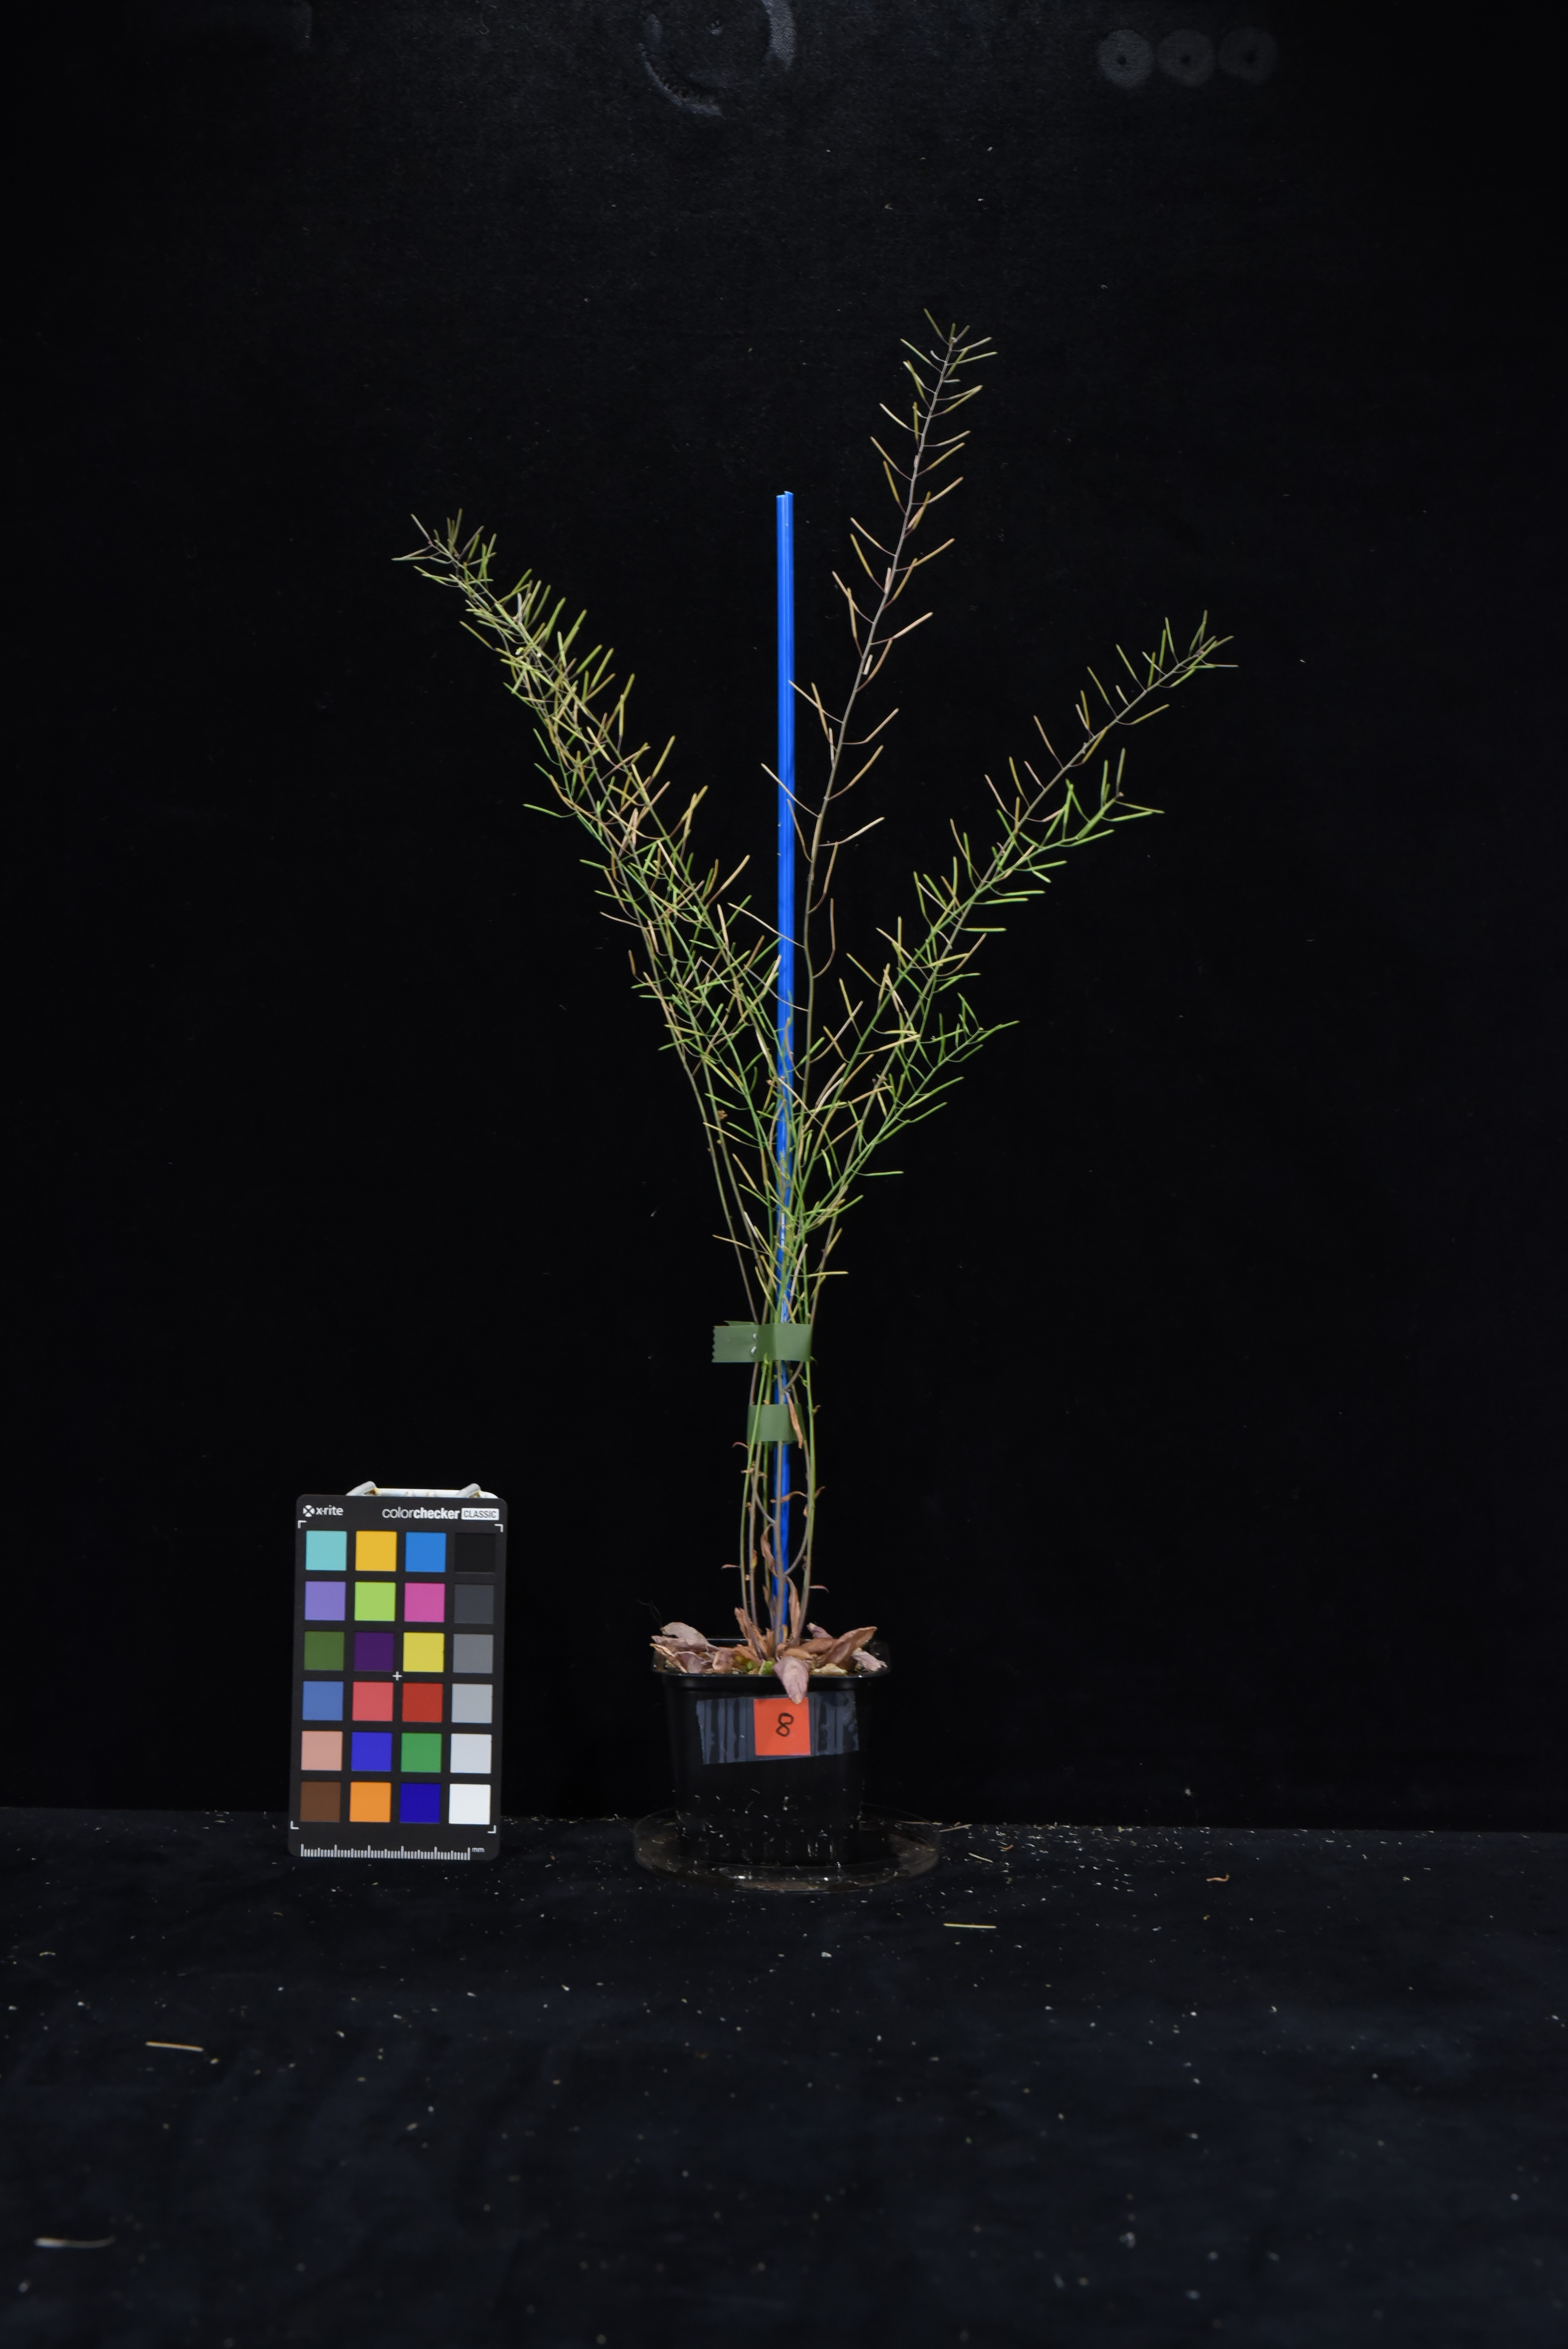
\includegraphics[width=0.3\linewidth]{20201029_8}
	 	\caption[Example image of a front-view image.]{An \textit{A. thaliana} plant during its reproductive phase (\textbf{after} binding the stems to a stick), imaged from the front. Just like the label, the stick should ideally be blue to facilitate separation from the plant itself in the analysis.}
	 	\label{fig:front_after}
	 \end{figure}
 
 \section{Image metadata\label{prep}}
 
 If we want to automate the image analysis, we need to make sure that each image contains all the metadata we need to assign the output to the correct plant. Imagine for example we take an image of a tray with 15 pots from the top and save that image as \texttt{DSC\_2487.JPG}. If we input this image into the analysis pipeline, it will output results for each of the 15 plants on the tray, which it will call \texttt{DSC\_2487.JPG\_1, DSC\_2487.JPG\_2} and so on. But what genotype is plant \texttt{DSC\_2487.JPG\_1} and how old was the plant when the picture was taken? The easiest way to embed metadata in your image is in the image name. If we for example rename our image \texttt{DSC\_2487.JPG} to \texttt{tray2\_day13.JPG}, the results for the first plant of the tray will we called \texttt{tray2\_day13.JPG\_1}, which we can very easily match to the tray layouts you have noted down. 
 
 You can rename the pictures by hand, but if you have followed my advice above and took the pictures always in the same order, we can also automate the renaming. The following script works on MacOS and Linux, and renames all \texttt{.JPG} files in the same folder. So create one folder with the picture from the top and one folder with the pictures from the front. The script renames the images with the day past germination and the number of each tray or plant. For example, if your plants germinated roughly on the 24th of July 2020, you'd set \texttt{germination=20200824}. If you have three full trays of plants, you would set the \texttt{end=3}  for the pictures taken from above, and \texttt{end=45} for the pictures of the individual plants taken from the front.
 
\begin{bashcode}
#!/bin/bash
# define the date of germination for DPG (days past germination) calculation
germination="20200824"
# number of the first sequentially numbered trays/plants
start=1
# number of the last sequentially numbered trays/plants
end=3
# rename images by DPG and tray/plant number
a=$start
for i in *.JPG; do
	var1="_"
	DPG=$(( ($(date -r "$i" +%s) - $(date --date=$germination +%s) )assign the starting 
		/ (60*60*24) ))
	mv -i -- "$i" "$DPG$var1$a.jpg"
	if [ "$a" -lt $end ]
	then
		let a=a+1
	else
		let a=$start
	fi
done
\end{bashcode} 

On Windows, you could install the bash shell as is described \href{https://www.howtogeek.com/249966/how-to-install-and-use-the-linux-bash-shell-on-windows-10/}{here}, to use the above script. Or you use the Python script below

\begin{pycode}
	## TODO: TRANSLATE BASH SCRIPT TO PYTHON
\end{pycode}

 
 \section{Image exploration in Fiji}
 
 To get a feeling for the images, open one of them in \href{https://imagej.net/Fiji/Downloads}{Fiji} and explore how you can segment and measure different parts of the plant. A very useful function for this is \texttt{Image} $\rightarrow$ \texttt{Adjust} $\rightarrow$ \texttt{Color Threshold...} (use the LAB colour space). To calibrate any height or area measurements, you can define the pixel size using the ruler on the bottom of the colour card.
 
 \section{High-throughput analysis in Python and PlantCV}
 
 You can do the complete analysis in Fiji, but depending on the amount of images you have, this might be prohibitively time consuming. The alternative is a programmatic approach that automates same principles of image analysis that we would use in Fiji. \href{https://plantcv.danforthcenter.org/}{PlantCV} is a Python library that was specifically designed for plant phenotyping. Getting started with it is more complicated than using Fiji, but once it is set up the reward is a highly reproducible analysis pipeline that needs minimal manual intervention. In the following I will outline the initial steps of working with our images in PlantCV. Beyond this short tutorial, I highly recommend the excellent official \href{https://plantcv.readthedocs.io/en/stable/}{documentation} of PlantCV. Lastly, if you are already familiar with PlantCV and want to skip ahead to the analysis pipeline optimised for our imaging setup, head over to my \href{https://github.com/leonardblaschek/plantcv}{Github page}.
 
 \subsection{Installation}
 
  I will assume that most students reading this document are using Windows 10. But even if not, most of what follows is operating system agnostic and will work (almost) identically on MacOS and Linux.
  
  \paragraph{Install Anaconda}
  \texttt{Anaconda} and its slimmed down version \texttt{Miniconda} are package and environment managers for Python. It allows you to create virtual environments for specific tasks, which simplifies work in Python immensely. If you do not have it installed already, I recommend \href{https://docs.conda.io/en/latest/miniconda.html}{\texttt{Miniconda}}. Simply follow the installation instruction for you operating system. If you are unsure, your operating system is almost definitely the 64-bit variant.
  
  \paragraph{Install PlantCV}
  If you are on Windows, start the \texttt{Anaconda Prompt}, on MacOS and Linux simply open a terminal window. To test that conda is properly installed, type:
  
 \begin{bashcode}
 	conda --version
 \end{bashcode}

The prompt should then output the installed conda version, for example \texttt{conda 4.9.2}. If this worked as expected, we next need to add the channel containing the PlantCV package to the conda configuration:

\begin{bashcode}
	conda config --add channels conda-forge
\end{bashcode}

Now we install PlantCV in a new environment called \texttt{plantcv}:

\begin{bashcode}
	conda create -n plantcv plantcv
\end{bashcode}

\subsection{Optimisation in Jupyter notebook}

\subsection{Batch analysis of multiple files}

\subsection{Data analysis}

\end{document}
